\section{PET Image Denoising}

%==================================================
\subsection{Image Denoising}
Image noise is a random variation of brightness and visible as grains. It may arise
by the sensor and circuity of a digital camera during the time of capturing or image
transmission that adds spurious and extraneous information \cite{verma2013comparative}. Noise in image
is defined as pixels showing false or different intensity values instead of true or
expected values. Natural image denoising is a process of reducing or removing
noise from an image. In other words, it is defined as a process of guesstimating an
original clean version of noise corrupted image \cite{levin2011natural}.

The common types of noise that arises in a image are impulse noise (salt-and-pepper
noise), amplifier noise (Gaussian noise), shot noise, quantization noise (uniform
noise), film grain, on-isotropic noise, multiplicative noise (speckle noise) and periodic
noise. Depending on owning different characteristics, which makes them
distinguishable, each type of noise is able to afflict image in different context. As
a result, noise reduction filters are developed to minimize the effects of noise in
order to ameliorate image processing.

In paper \cite{hanzouli2013pet}, the developed framework was firstly evaluated for \gls{pet} denoising. In this work the multiobservation
aspect of the proposed \gls{hmt} was exploited in
order to associate both Wavelets and Contourlets coefficients
to each voxel. An approach combining both \gls{cd} and \gls{wd}, namely \gls{wcd}, was proposed in order to obtain the optimal performance.


%==================================================
\subsection{PET Image}
\gls{pet} is a nuclear medicine, functional imaging technique that is used to observe metabolic processes in the body. The system detects pairs of gamma rays emitted indirectly by a positron-emitting radionuclide (tracer), which is introduced into the body on a biologically active molecule. 

Three-dimensional images of tracer concentration within the body are then constructed by computer analysis. In modern PET-CT scanners, three dimensional imaging is often accomplished with the aid of a CT X-ray scan performed on the patient during the same session, in the same machine.

The examples of \gls{pet} system and \gls{pet} brain image can be seen in Figure \ref{fig:pet_image}.

\begin{figure}[h]
	\centering
	\begin{subfigure}[b]{0.45\textwidth}
		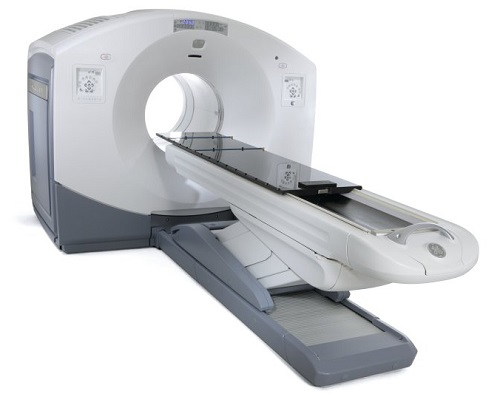
\includegraphics[width=\textwidth]{fig/pet_machine.jpg}
		%\caption{\gls{pet} machine}
		\label{fig:pet_machine}
	\end{subfigure}
	\begin{subfigure}[b]{0.35\textwidth}
		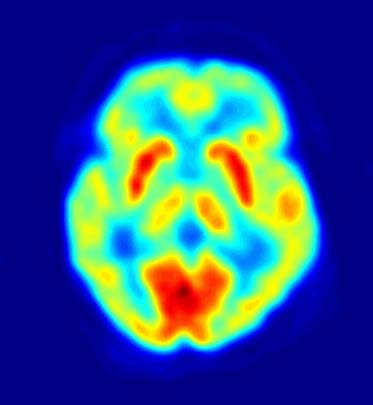
\includegraphics[width=\textwidth]{fig/pet_brain.jpg}
		%\caption{\gls{pet} brain image}
		\label{fig:pet_brain}
	\end{subfigure}
	\caption[PET Denoising - \gls{pet} system and \gls{pet} brain image]{PET system and brain image}\label{fig:pet_image}
\end{figure}


%==================================================
\subsection{Wavelet and Contourlet Denoising}
\label{subsection:wavelet_denoising}

%--------------------------------------------------
\subsubsection*{Wavelet denoising}
Wavelet thresholding methods for noise removal, in which the wavelet coefficients are
thresholded in order to remove their noisy part, were first introduced by Donoho in 1993 \cite{coifman1995translation}.
The theoretical justifications and arguments in their favour are highly compelling. These
methods do not require any particular assumptions about the nature of the signal, permits
discontinuities and spatial variation in the signal, and exploits the spatially adaptive
multiresolution of the wavelet transform \cite{cohen2012signal}.

%--------------------------------------------------
\subsubsection*{Contourlet Denoising}
The major drawback for wavelets in two-dimensions is
their limited ability in capturing directional information. To
overcome this deficiency, researchers have recently considered multiscale and directional representations that can capture the
intrinsic geometrical structures such as smooth contours in
natural images \cite{Po2003}.

The primary goal of the contourlet construction is to obtain a sparse expansion for typical images that
are piecewise smooth away from smooth contours \cite{do2005contourlet}.

%--------------------------------------------------
\subsubsection*{Concept of denoising}

\begin{figure}[h]
	\centering
	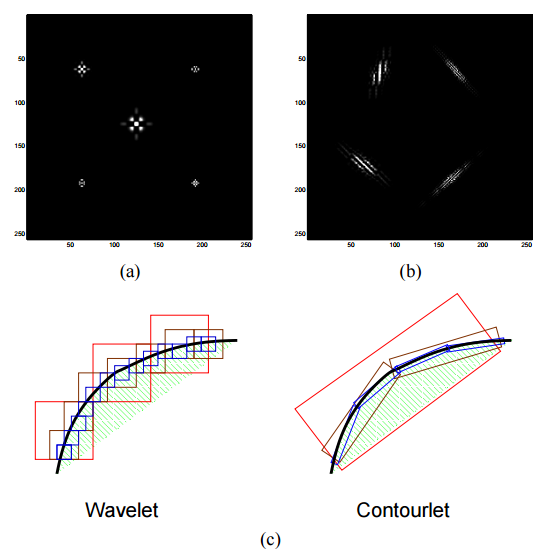
\includegraphics[width=0.7\textwidth]{fig/wavelets_contourlet}
	\caption[PET Denoising - Comparison between Wavelet and Contourlet]{Contourlet and wavelet representations for images. (a) Examples of
		five 2-D wavelet basis images. (b) Examples of four contourlet basis images.
		(c) Illustration showing how wavelets having square supports that can only
		capture point discontinuities, whereas contourlets having elongated supports
		that can capture linear segments of contours, and thus can effectively represent
		a smooth contour with fewer coefficients.
	}
	\label{fig:wavelets_contourlet}
	
\end{figure}

A more precise explanation of the wavelet denoising
procedure can be given as follows. Assume that the
observed data is \cite{rangarajan2002image}:
\begin{equation}
X(t)=S(t)+N(t)
\end{equation}
where $S(t)$ is the uncorrupted signal with additive
noise $N(t)$. 

Let $W(\cdot)$ and $W^{-1}(\cdot)$ denote the forward
and inverse wavelet transform operators. Let $D(\cdot, \lambda)$ denote the denoising operator with threshold $\lambda$. 

We intend to denoise $X(t)$ to recover $\hat{S}(t)$ as an estimate
of $S(t)$. The procedure can be summarized in three
steps:
\begin{subequations}
	\begin{align}
	Y &= W(X)\\
	Z &= D(Y,\lambda)\\
	\hat{S} &= W^{-1}(Z)
	\end{align}
	\label{eqn:wavelet_denoise}
\end{subequations}
while $D(\cdot,\lambda)$ being the thresholding operator and $\lambda$ being the threshold.

%--------------------------------------------------
\subsubsection*{Thresholding}
In fact, small coefficients are dominated by noise, while coefficients with a large absolute value carry more signal information than noise. Replacing noisy coefficients (small coefficients below a certain threshold value) by zero and an inverse wavelet transform may lead to a reconstruction that has lesser noise \cite{rangarajan2002image}. 

There are three kinds of thresholding for denoising:
\begin{itemize}
	\item Hard thresholding
	\item Soft thresholding
	\item Universal thresholding
\end{itemize}

\begin{figure}[h]
	\centering
	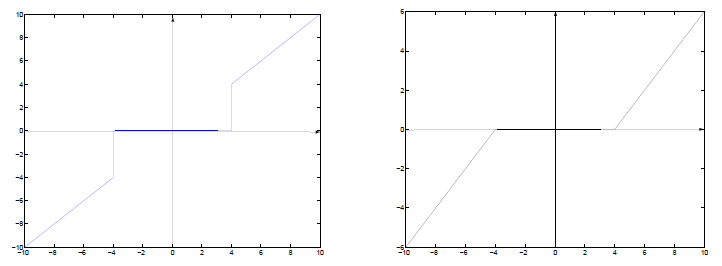
\includegraphics[width=0.8\textwidth]{fig/hard_soft_thresholding}
	\caption[PET Denoising - Hard and Soft Thresholding]{Hard and Soft Thresholding}
	\label{fig:hard_soft_thresholding}
\end{figure}

Hard threshold is a "keep or kill" procedure and
is more intuitively appealing. The alternative, soft
thresholding shrinks coefficients above the threshold in absolute value. See Figure \ref{fig:hard_soft_thresholding} for the transfer functions of hard and soft thresholding, respectively. 

The hard thresholding operator is defined as:
\begin{equation}
D(U, \lambda) = 
\begin{cases}
U &\text{for all $|U|>\lambda$ }\\
0 &\text{otherwise}
\end{cases}	
\end{equation}

Otherwise, the soft thresholding operator is defined as:
\begin{equation}
D(U, \lambda) = sgn(U)max(0, |U| - \lambda)
\end{equation}

Threshold determination is an important question when denoising. A small threshold
may yield a result close to the input, but the
result may still be noisy. A large threshold on the other hand, produces a signal with a large number
of zero coefficients. This leads to a smooth signal.
Paying too much attention to smoothness, however,
destroys details and in image processing may cause
blur and artifacts \cite{rangarajan2002image}.

In addition to hard and soft thresholding, a thresholding approach, namely universal thresholding, is introduced:
\begin{equation}
\lambda_{UNIV}=\sqrt{2lnN\sigma}
\end{equation}
where $N$ being the signal length, and $\sigma^2$ being the noise variance.


%==================================================
\subsection{Wavelet-Contourlet Denoising}

On the one hand, Wavelet based methods exploit observation-based transforms at different resolutions in order to better describe the whole observed information. The major drawback of Wavelets is their limited ability in
capturing directional information. 

On the other hand, the \gls{ct} has emerged as an efficient tool able
to capture the intrinsic geometrical structures such as smooth
contours thanks to a high degree of directionality and
anisotropy. This transform is however not optimal for isotropic
structures, contrary to Wavelets.

Consequently, an approach combining both transforms may
lead to optimal performance. In this work the multiobservation
aspect of the proposed \gls{hmt} was exploited in
order to associate both Wavelets and Contourlets coefficients
to each voxel, leading to a Wavelet-Contourlet
Denoising (WCD).


\begin{figure}[h]
	\centering
	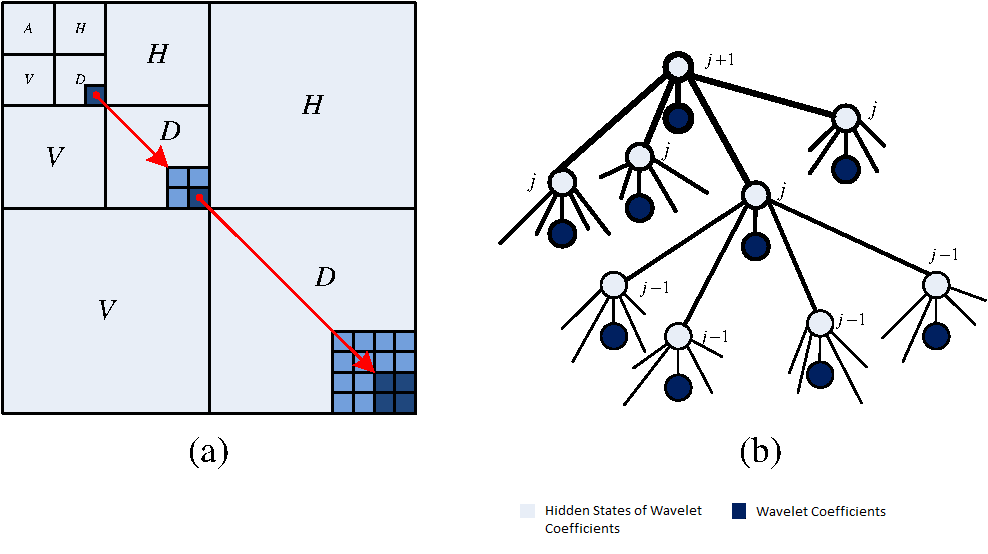
\includegraphics[width=0.8\textwidth]{fig/wavelets_hmt}
	\caption{\glsdesc{dwt} and \glsdesc{hmt} models}
	\label{fig:wavelets_hmt}
\end{figure}


%==================================================
\subsection{Proposed denoising method: Non-local Means}
%--------------------------------------------------
%\subsubsection*{Background}

\gls{nlm} is a linear smoothing technique introduced by \citeauthor{buades2005non}. \gls{nlm} filtering
is an algorithm computing average values of all pixels in the image, which are analyzed
how similar they are to the objective pixel. The main difference between \gls{nlm} and other filters is the meticulous employment of all possible self-predictions
an image is able to provide.

Compared to local filters, which process pixels within a local square window to aim
for a reconstruction of the main geometrical configurations, \gls{nlm} is more effective
in post-filtering intelligibility and preserving details of image and fine structure \cite{buades2005non}.


%==================================================
\subsection{Proposed denoising method: Sparse 3D Transform-domain Collaborative Filter}
%--------------------------------------------------
%\subsubsection*{Background}
Currently, \gls{bm3d} is a well-known
image denoising algorithm introduced by \citeauthor{dabov2007image} in 2007 \cite{dabov2007image}. The basic principles
of this algorithm is grouping and collaborative Wiener filtering in two-stage
estimations. There is a number of developed algorithms based on the concepts of
BM3D; however, BM3D is still the most successful
approach, especially for low-SNR \gls{pet} image.



%\footnote{An example footnote.}